\section{Interferenz und Beugung}
\textbf{Interferenz:} Überlegung von Wellen, die statische Intensitätsmuster erzeugt. \\
\textbf{Beugung:} Abweichung der Wellenausbreitung von geometrischer Strahlrichtung an Öffnung oder Hindernis

\subsection{Phasendifferenz und Kohärenz}
Überlagerung zweier em-Wellen \\[1ex]
\hspace{5mm} $E_1 = E_0 \sin{(kx_1 - \omega t + \delta_1)}$ \\
\hspace{5mm} $E_2 = E_0 \sin{(kx_2 - \omega t + \delta_2)}$ \\[1ex]
\textbf{Differenz der Phasen beider Wellen} (zum Zeitpunkt $t$):

\begin{formulabox}
    \[
        (kx_1 - \omega t + \delta_1) - (kx_2 - \omega t + \delta_2) = k(x_1 - x_2) - \delta = k \cdot \Delta r - \delta
    \]
\end{formulabox}
    $\Delta r$: Wegunterschied / Gangunterschied \\[1ex]

\textbf{Konstruktive Interferenz:}
\[
    k \cdot \Delta r - \delta \hspace{3mm} \text{ganzzahliges Vielfaches von $2\pi$}
\]
\begin{center}
    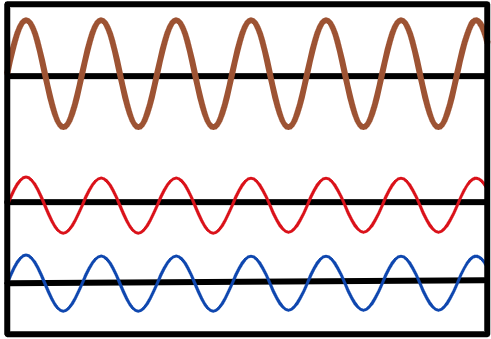
\includegraphics[width=0.18\linewidth]{Abbildungen Physik ZF/Konstruktive Interferenz.png}
\end{center}

\textbf{Destruktive Interferenz:}
\[
    k \cdot \Delta r - \delta \hspace{3mm} \text{unganzzahliges Vielfaches von $\pi$}
\]
\begin{center}
    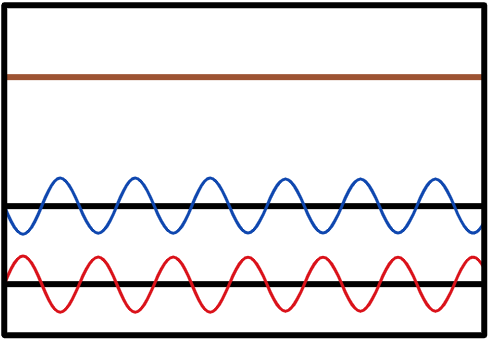
\includegraphics[width=0.18\linewidth]{Abbildungen Physik ZF/Destruktive Interferenz.png}
\end{center}

\textbf{Kohärenz:}
feste Phasenbezeichung \\
Allgemeiner: \textbf{"Interferenzfähigkeit"} \\
\hspace{5mm} Vorraussetzung: gleiche Polarisation \& Wellenlänge \\[1ex]

\subsection{Interferenz an dünnen Schichten}
\textbf{Phasenunterschied:}
\[
    \Delta = \frac{2 \pi}{\lambda'} \cdot 2s - \pi = \frac{2\pi}{\lambda} \cdot 2sn - \pi
\]

\textbf{Konstruktive Interferenz,} wenn:

\begin{formulabox}
    \[
        \Delta = m \cdot 2\pi \hspace{7mm} m = 0,  \pm 1, \pm 2, \dots
    \]
\end{formulabox}
    \hspace{5mm} $\rightarrow \lambda(m+\frac{1}{2}) = 2sn$ \\[1ex]
\textbf{Destruktive Interferenz,} falls:

\begin{formulabox}
    \[
        \Delta = (2m + 1)\pi \hspace{5mm} m = 0,  \pm 1, \pm 2, \dots
    \]
\end{formulabox}
    \hspace{5mm} $\rightarrow m\lambda = 2sn$ \\[1ex]

$\Rightarrow$ Streifenmuster durch Variation der Dicke $s$, \\ 
\hspace{3mm} bunte Streifen wegen Abhängigkeit von $\lambda$

\subsection{Interferenzmuster beim Doppelspalt}
Ann.: Die Wege des Lichts von den beiden Spalten zum Punkt $P$ auf dem Schirm können als parallel betrachtet werden. \\[1ex]
Für die Interferenz ist nur der Gangunterschied $d \cdot \sin{\Theta}$ entscheidend. \\[1ex]

\textbf{Intensitätsminima} (destruktiv):

\begin{formulabox}
    \[
        d \cdot \sin{\Theta} \Rightarrow \left(m + \frac{1}{2}\right) \lambda \hspace{5mm} m = 0,  \pm 1, \pm 2, \dots
    \]
\end{formulabox}

\textbf{Intensitätsmaxima} (kontruktiv):

\begin{formulabox}
    \[
        d \cdot \sin{\Theta} \Rightarrow  m\lambda \hspace{7mm} m = 0,  \pm 1, \pm 2, \dots
    \]
\end{formulabox}

\textbf{Für kleine Winkel $\Theta$ gilt:} $\sin{\Theta} = \tan{\Theta} = \frac{y}{l}$

\begin{formulabox}
    \[
        \Rightarrow y_m \approx m \cdot \frac{yl}{d} \hspace{5mm} \text{Position des m-ten Maximums}
    \]
\end{formulabox}

\textbf{Berechnung der Intensität auf dem Schirm:} \\[1ex]

\hspace{3mm} Welle von Spalt 1 zu Punkt $P$:
\[
    E_1 = A_0 \sin{\alpha} \hspace{10mm} \text{mit } \alpha = kx - \omega t
\]
\hspace{3mm} Welle von Spalt 2 zu Punkt $P$:
\[
    E_2 = A_0 \sin{(\alpha + \delta)} \hspace{7mm} \text{mit } \delta = k \cdot \Delta r = \frac{2\pi}{\lambda} \cdot d \sin{\Theta}
\]

\hspace{3mm} Aus \textbf{Überlagerung} resultierende Welle:

\begin{formulabox}
    \[
        E = E_1 + E_2  = \underbrace{2 A_0 \cos{ \left(\frac{1}{2}\delta \right)}}_{\text{Amplitude $E_0$ der Gesamtwelle}} \cdot \sin{\left( \alpha + \frac{1}{2}\delta \right)}
    \]
\end{formulabox}

\hspace{3mm} Intensität:

\begin{formulabox}
    \[
        I = |E_0|^2 = 4 A_0^2 \cos^2{\left(\frac{1}{2}\delta \right)}
    \]
\end{formulabox}

\subsection{Beugung am Gitter}
\textbf{Interferenzmaxima} zweier benachbarten Spalten liegen bei:

\[
    g \cdot \sin{(\Theta_m)} = m\lambda \hspace{7mm} m = 0,  \pm 1, \pm 2, \dots
\]

Das Gitter besitzt eine grosse Anzahl beleuchteter Spalten $N$. Das nächste Minium befindet sich dort, wo der Gangunterschied zwischen dem \textbf{mittleren Spalt $\frac{N}{2}$ und dem ersten Spalt $\frac{\lambda}{2}$} beträgt. (analog: 2. Spalt $\frac{N}{2} + 1$, usw.) \\[1ex]

\textbf{Der Abstand zwischen den beiden Spalten beträgt:}
\[
    \left( \frac{N}{2} - 1 \right) g \approx \frac{N}{2}g \hspace{10mm} \text{Ann.: $N$ ist gross} 
\]
\[
    \Rightarrow \frac{N}{2}\sin{(\Theta_{min})} = \frac{\lambda}{2} \hspace{10mm} \sin{(\Theta_{min}) \approx \Theta_{min} = \frac{\lambda}{N \cdot g}}
\]
\textbf{Breite der Maxima beim Gitter mit $N$ Spalten:}

\begin{formulabox}
    \[
        \Delta \Theta = 2 \Theta_{min} = \frac{2 \lambda}{N \cdot g}
    \]
\end{formulabox}
 
\hspace{5mm} $\rightarrow$ viele beleuchtete Spalten $\Rightarrow$ schmale Maxima \\
\hspace{5mm} $\Rightarrow$ gute Trennung unterschiedlicher Wellenlängen \hspace{1mm} (Anwendung: Spektrometer)

\subsection{Beugung beim Einzelspalt}
Im Intensitätsminimum löschen sich der Mittelstrahl und ein Strahl vom Rand des Spalts gegenseitig aus. Daraus folgt: 

\[
    \underbrace{\frac{1}{2}a  \cdot \sin{(\Theta_1)}}_{\text{Gangunterschied}} = \underbrace{\frac{1}{2}\lambda}_{\text{Bedingung für destruktive Interferenz}}
\]

\begin{formulabox}
    \[
        \sin{(\Theta_1)} = \frac{\lambda}{a}
    \]
\end{formulabox}

\textbf{Analog findet man für die weiteren Minima:}

\begin{formulabox}
    \[
        \sin{(\Theta_m)} = m \frac{\lambda}{a} \hspace{7mm} m = 0,  \pm 1, \pm 2, \dots
    \]
\end{formulabox}

\subsection{Beugung und Auflösung}
\textbf{Betrachtung:} Beugung an einem kreisrunden Öffnung mit Durchmesser $D$ \\[1ex]

Winkel unter dem das \textbf{erste Intensitätsminimum auftritt:}

\begin{formulabox}
    \[
        \sin{(\Theta)} = 1.22 \frac{\lambda}{D}
    \]
\end{formulabox}

\textbf{Für kleine Winkel:}

\begin{formulabox}
    \[
        \Theta = 1.22 \frac{\lambda}{D} \hspace{5mm} \text{oder. } \frac{x}{h}
    \]
\end{formulabox}

Dient als Kirterium für das Auflösungsvermögen eines Instruments \textbf{(Rayleigh Kriterium)}
